% !TEX root = ../main.tex
\section{General Overview}

This document presents the design of a configurable, precise current source for use in cranial impedance measurements. The device is designed to produce an isolated current source capable of outputting sinusoidal, triangle, or square wave modulated current with user-selectable frequencies ranging from $50$Hz to $100$KHz with user selectable peak to peak amplitudes between $500$nA and $200$uA. The device is also capable of direct current injection in the same amplitude range. A modular multiplexer installed between the current source and the output allows for interfacing with up to 1024 individual probes, with this design specification document describing the 256 probe configuration. Both the forward and return probe are individually selectable. A diagram showing the general layout of the device is shown in Fig \ref{fig:generaldiagram}. 

\begin{figure*}[!htb]
\centering
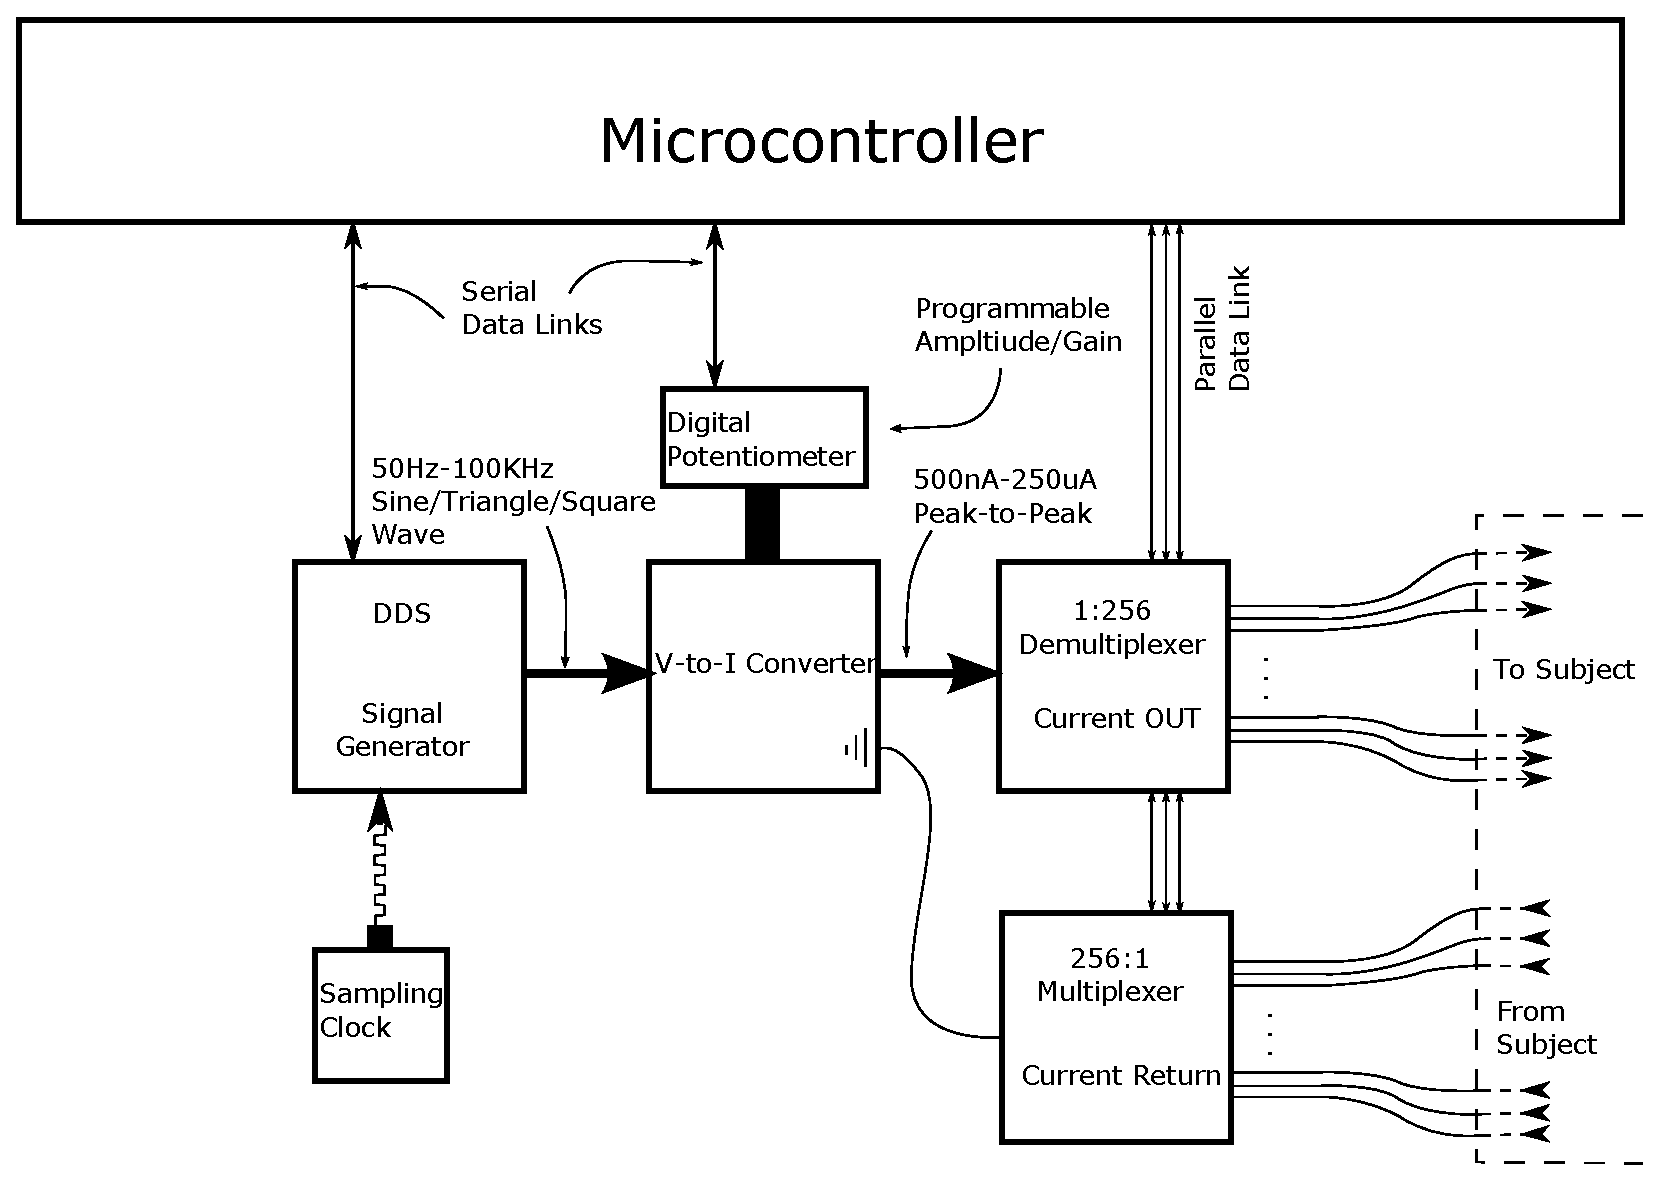
\includegraphics[width=\linewidth]{images/generaldiagram/current.eps}
\caption{A diagram of the device. A Direct Digital Synthesis (DDS) Integrated circuit generates the signal source with programmable output shape (Sinusoidal, Triangle, or Square wave output) and frequency ($50$Hz to $100$KHz with resolution $<1$Hz). The DDS output is fed into a Voltage to Current conversion circuit to generate the stable current source to drive the TDCS, A digital potentiometer selects the gain and is used to adjust the amplitude of the current source. The current is then fed into a digitally controlled demultiplexer (digital switch) that selects the output channel, an independently controlled multiplexer selects the return channel. A microcontroller or computer with general digital input/output capabilities is used to control the device through serial and parallel data links. An independent sampling clock generates the clock signal to run the DDS. All communications with the micro controller are buffered to isolate the noisy digital circuitry from the current source and to allow for flexibility in the choice of microcontroller}
\label{fig:generaldiagram}
\end{figure*}

The application specifications require a user programmable, low-noise, precise current source for driving the current injection probes. The following subsections describe the theory of operation of each block in the current driver circuitry. 

\subsection{DDS}
There are several options for generating the signal source for the current driver. Analog only options include using an oscillator and resonator circuit to generate the sine wave, or an operational amplifier circuit capable of self-oscillation like a Wien-Bridge resonator. Digital options include having a micro controller or FPGA driving a Digital-to-Analog Converter (DAC) with the right sequence of codes in order to generate the desired signal. A "Direct Digital Synthesis" (DDS) Integrated Circuit (IC) is a single chip solution that is designed for low noise and high precision generation of sinusoidal waveforms (due to the nature of the generator circuit triangle and square wave outputs are automatically available as well). An FPGA or micro controller based solution has the benefit of arbitrary signal generation, however due to the isolated nature of the current source, it would require placing the noisy digital circuitry with the sensitive analog circuitry, undesirable in this application. 

Commercially available DDS IC's have 24 to 32-bit wide "frequency words" allowing for sub-hertz precision in frequency selection in a standard configuration, with an integrated 10-12 bit DAC to drive the output. DDS IC's are typically designed for telecom applications, where generated frequencies are in the megahertz range and are optimized for low frequency noise at these high frequencies, in audio frequency range applications this means exceptional frequency stability in the parts-per-billion range. The current design employs a AD9838 DDS IC from Analog Devices [CITE].

The AD9838 and similar DDS IC's employ a "complimentary current" output stage rather than a pure voltage output DAC. In high speed applications, the large resistive losses encountered when trying to "swing" the DAC output from one voltage extreme to another can be detrimental in high speed applications. At this speed this effect is negligible, but complementary current outputs provide a convenient way of coupling with the Current driver. A schematic of the DDS stage is shown in figure \ref{fig:dds-stage}

\subsection{Voltage to Current Converter}

The current driver is designed around the use of a instrumentation amplifier to sense the voltage generated when the DDS drives its current directly to ground across a small resistance. The instrumentation amplifier provides a convenient way to AC couple the output DAC of the DDS for a symmetrical AC signal (rather than the DC offset signal that the DAC outputs), while simultaneously acting as a precision current source, and with a programmable gain easily selectable by a resistor or, in this case, a digital potentiometer. The instrumentation amplifier was chosen for its convenient gain selection and excellent common-mode rejection. 

A separate, high bandwidth and fast slew operational amplifier is used to drive the instrumentation amplifier as a precise current source. A resistor is used to set the current level for a given input voltage, with a (non-digital) trim-potentiometer used for callibration. 

In the current configuration with $\pm15$V source voltages for the instrumentation amplifier, the current driver can be used to drive currents from $500$nA to $100\mu$A in 3 selectable range configurations. 


\subsection{Output Switching}

The target EIT system employs a 256 probe mesh on the subject. In order to allow arbitrary selection in both source and drain probe  two independent 256:1 de/multiplexers are required, There are no commercially available analog multiplexers with 256 outputs, so a tree of 32:1 multiplexers is required to accomplish the switching. Analog multiplexers are characterized by their leakage current (how much of the input leaks into the outputs that are not selected), their forward resistance, and their switching speed.Analog multiplexers typically are bidirectional, so they work equally well as multiplexers (many to one) and demultiplexers (one to many).  ADG732 multiplexers were chosen as they accommodate large switch counts (32:1), have very low forward resistance, fast switching speed, and ultra low leakage current.

In order to accommodate the 512 input and output connections, the multiplexers are split onto modular pc-boards, each accommodating 64 inputs and outputs (input and output lines are shared as the probes used are the same). The digital control signals are propagated to each board along shared signal lines, so in this configuration only one input and output are selectable at once, in further revisions, multiple current return paths and the option for multiple current sources may be developed.



 






